\documentclass[12pt,a4paper]{article}

\usepackage[default]{opensans}
\usepackage{amsfonts}
\usepackage{amsmath}
\usepackage{amssymb}
\usepackage{graphicx}
\usepackage[numbers,sort&compress]{natbib}
\usepackage{epsfig}
\usepackage[usenames,dvipsnames]{xcolor}
\usepackage{array}
\usepackage{url}
\usepackage[nottoc,numbib]{tocbibind}
\usepackage[format=plain,
            labelfont={bf,it},
            textfont=it]{caption}

\definecolor{myblue}{RGB}{25,25,112}

\usepackage[colorlinks=true
,urlcolor=myblue
%,urlcolor=black
,anchorcolor=myblue
,citecolor=myblue
,filecolor=myblue
,linkcolor=myblue
,menucolor=myblue
,linktocpage=true
,pdfproducer=medialab
,bookmarks=false]{hyperref}
%\usepackage{slashed}

\topmargin      -0.5in  % distance to headers
\headheight      0.2in  % height of header box
\headsep         0.3in  % distance to top line
\textheight      9.25in  % height of text
\footskip        0.3in  % distance from bottom line
\oddsidemargin   0.0in  % Horizontal alignment
\evensidemargin  0.0in  % Horizontal alignment
\textwidth       6.25in  % Horizontal alignment	


% Lengths ----------------------------------------------------------------------

% save parindent to a new length, originalparindent
\newlength{\originalparindent}
\setlength{\originalparindent}{\parindent}

% set parskip to bigskipamount for space between paragraphs
\setlength{\parskip}{\bigskipamount}

% set parindent to 0pt for disabling paragraph indentation
\setlength{\parindent}{0pt}





\date{}

\begin{document}

\thispagestyle{empty}

\begin{center}

\textsf{}

\vskip 1.2cm

{\LARGE \bf Fire Emergencies in Seattle}

\vskip 0.1cm

{\Large Correlations with Rain Patterns and Human Activity}
 

\vskip 0.75cm

{\bf \large S.~C.~Vargas}
%\let\thefootnote\relax\footnote{{\tt secavara@gmail.com}}\\

%\vskip 25pt

%{\em Department of Physics and Astronomy, Uppsala University, \\ Box 516, SE-751 20 Uppsala, Sweden \\}

\end{center}

\vskip 1cm


\begin{figure}[ht!]
\centering
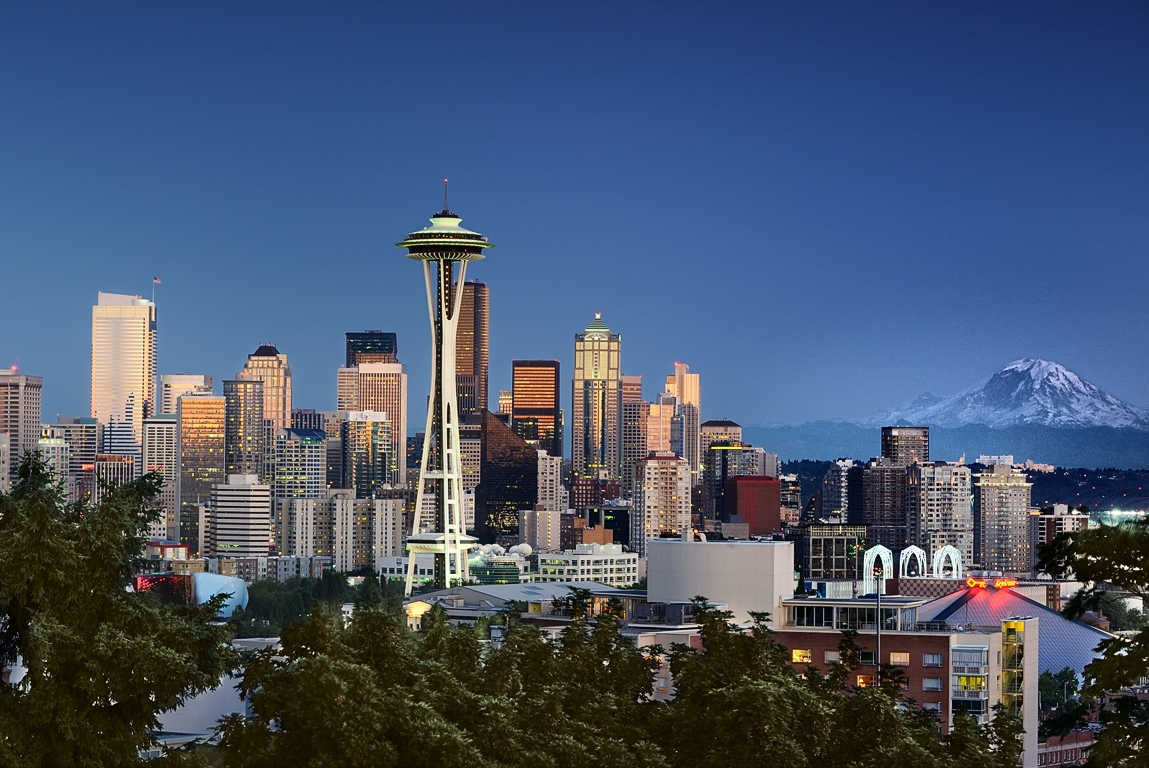
\includegraphics[scale=0.5]{figs/Seattle_Pic.jpg}
%\caption{ }
\label{pic}
\end{figure}
\vspace{-0.8cm}
\begin{center}
{\small License notice: \href{https://www.flickr.com/people/43518209@N00}{Bala} from Seattle, USA, \href{https://commons.wikimedia.org/wiki/File:Seattle_from_Kerry_Park_(1).jpg}{Seattle from Kerry Park (1)}, \href{https://creativecommons.org/licenses/by/2.0/legalcode}{CC BY 2.0}.}
\end{center}

%\begin{center}
%{\bf ABSTRACT}\\[3ex]
%\begin{minipage}{13cm}
%\small
%This is an abstract. This is an abstract. This is an abstract. This is an abstract. This is an abstract. This is an abstract. This is an abstract. This is an abstract. This is an abstract. This is an abstract. This is an abstract. This is an abstract. This is an abstract. This is an abstract. This is an abstract. This is an abstract. This is an abstract. This is an abstract. This is an abstract. This is an abstract. This is an abstract. This is an abstract. This is an abstract. This is an abstract. This is an abstract. This is an abstract. This is an abstract. This is an abstract. This is an abstract. This is an abstract. This is an abstract. This is an abstract.
%\end{minipage}
%\end{center}

\newpage

\tableofcontents

\newpage

\section{Problem}

Can we establish trends in 911 fire calls in Seattle to predict and find patterns, or correlate them with factors such as rain patterns?

\section{Client(s)}

Governmental agencies might be interested in this study to refine strategies that pin point influential factors in the manifestation of fires in Seattle. Insurance agencies might also find this relevant. Ultimately, the objective is to reduce the significant human and financial cost generally associated with fires. Reducing the number of fires will ultimately allow the police, fire department and other dependencies to divert their resources in other issues faced by the city and its inhabitants.

\section{Sources and Data Sets}


{\large \href{https://www.kaggle.com/city-of-seattle/seattle-observed-monthly-rain-gauge-accumulations/version/16}{Seattle Observed Monthly Rain Gauge Accumulations} \cite{Daniels2018}}

These monthly data goes from October 2002 to May 2017, containing measurements of 17 rain gauges located throughout Seattle city limits. There is no information on the units describing the amounts of rain. The locations of the rain gauges are given indirectly in a image (see Figure~\ref{gauges}).

Freely available for download, modification and distribution, under the license \href{https://creativecommons.org/publicdomain/zero/1.0/legalcode}{CC0 1.0}.

\begin{figure}[ht!]
\centering
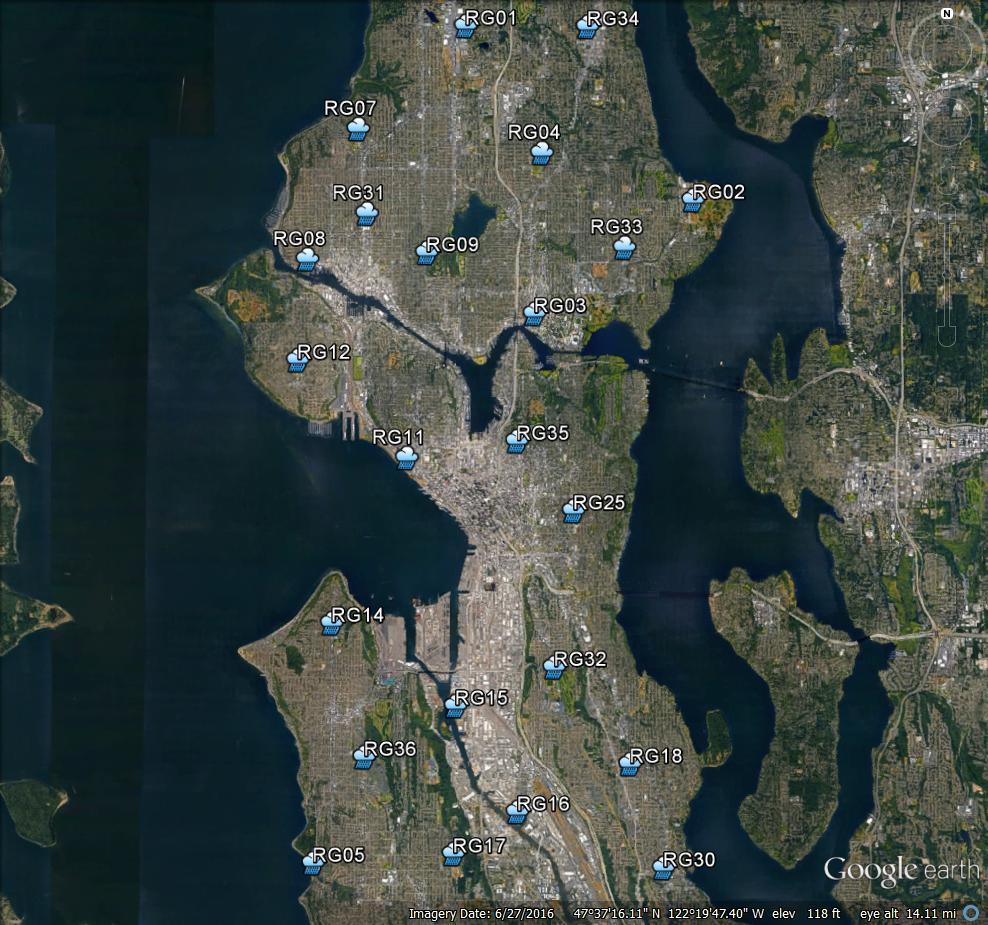
\includegraphics[scale=0.3]{figs/SPU_DWW_RGs.jpg}
\caption{Locations of rain gauges in Seattle. In reality, measurements for only 17 of these gauges are reported. This image is part of the data set in \cite{Daniels2018}.}
\label{gauges}
\end{figure}



{\large \href{https://data.seattle.gov/Public-Safety/Seattle-Fire-911-Calls-from-3-1-2010-to-3-1-2011/d9j6-s59d}{Seattle Fire 911 Calls} \cite{FireData2018}}

Fire 911 calls in Seattle, from 2010 to 2011. It contains latitude and longitude of the location of the caller, in addition to date, time and type of call. This version corresponds to the September 2, 2018 update.

Freely available for download, modification and distribution, under the license \href{https://creativecommons.org/publicdomain/zero/1.0/legalcode}{CC0 1.0}.

{\large Holidays in Washington State in \href{https://www.officeholidays.com/countries/usa/regional.php?list_year=2010&list_region=washington}{2010} and \href{https://www.officeholidays.com/countries/usa/regional.php?list_year=2011&list_region=washington}{2011} \cite{OfficeHolidays2010,OfficeHolidays2011}}

Federal and state holidays in 2010 and 2011 in the state of Washington. These were retrieved in October 10, 2018.

\section{Data Wrangling and Exploratory Data Analysis}

\subsection{Rain Data Set}

With the help of Figure~\ref{gauges}, we can deduce an approximate location for the rain gauges (latitude and longitude) which we store in a dictionary. As we mentioned, only 17 rain gauges actually appear in the data set.

We proceed to import the \verb|csv| file and read it as a data frame. The data has a date column, and a column for each 17 rain gauges. The date column shows that measurements were taken monthly, while the other columns indicate values for rain accumulation (in unknown units). These cover the period from November, 2002 to May, 2017.

We first proceed to search for null values or outliers. There are no null or non-existent values in the set and a direct plotting of all the data shows it to be fairly reasonable between the expectations of seasonal behavior. For instance, we can see this in the case of the gauge RG01, as shown in Figure~\ref{RG01_Full}.

\begin{figure}[ht!]
\centering
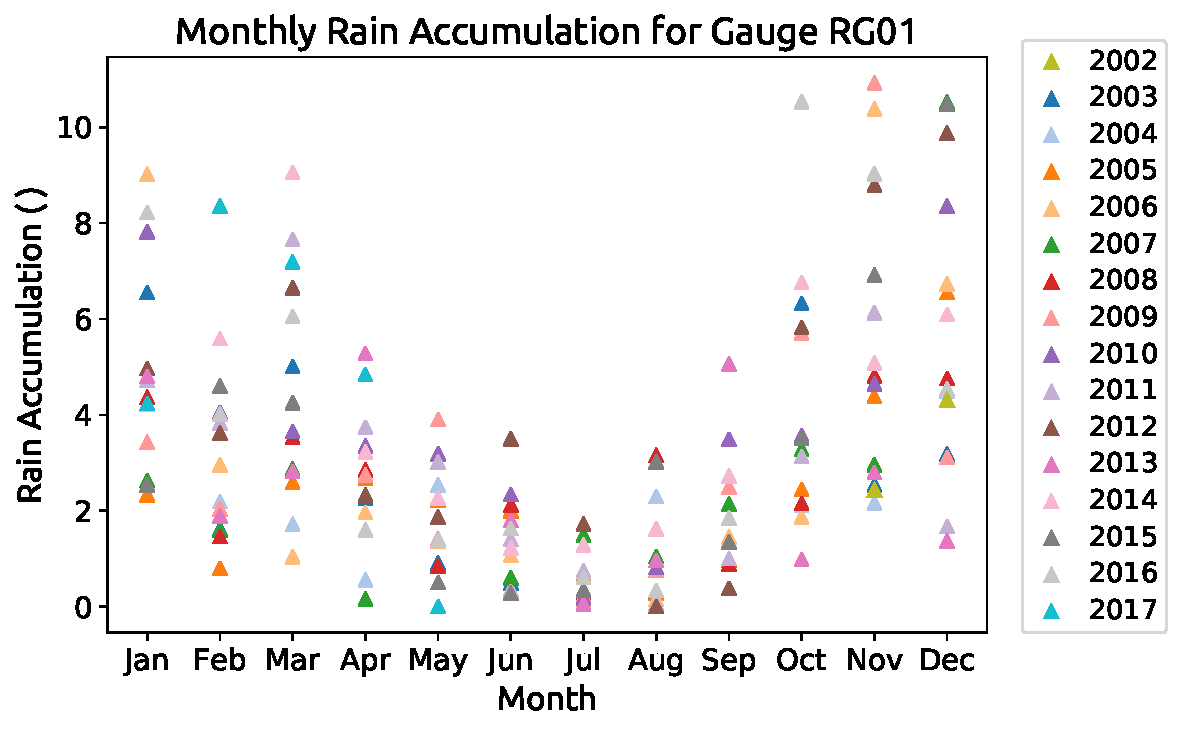
\includegraphics[scale=0.6]{figs/RG01_Full.pdf}
\caption{Rain accumulations measured by the gauge RG01 for all years.}
\label{RG01_Full}
\end{figure}

We are interested in the correlation between these weather data and the frequency of fire emergency calls. The fire 911 calls set covers only the period between 2010-07 and 2011-02, so we select the rain data corresponding to this interval in a separate data frame which we label \verb|df_rain_10_11_F|.

\subsection{Fire 911 Calls}

Let us consider the 911 fire calls set. We can import it directly from the Seattle data website and read it as a data frame. It has 4 columns: \verb|Type| of the call, \verb|Datetime|, \verb|Latitude| and \verb|Longitde| of the caller. It has no null values.

In order to see if the fire 911 data is correlated to the rain patterns, we have to associate their location with the location of the rain gauges. In order to do this, we write two functions:

\begin{verbatim}
great_circle_dist(lat1,lon1,lat2,lon2) 
\end{verbatim}

which computes the distance in kilometers between two points, given their latitude and longitude, and

\begin{verbatim}
closest_g(lat,lon) 
\end{verbatim}

which picks a point and finds the closest rain gauge. By using the latter, we can find the nearest gauge to each 911 caller. Effectively, this defines rain gauge regions as partitions or sectors that cover the city of Seattle. In a way, we are using a nearest neighbor approach indirectly. 

We add a new column to the fire 911 calls data frame, \verb|C_gauge|, which gives the nearest rain gauge. In addition, by taking a look of the \verb|Type| column, we see that not all calls are explicitly related to fires. We select here the calls that have \verb|'Fire'| in the \verb|Type| description.

We build a new data frame where we keep only the \verb|Datetime| and the closest gauge of these Fire calls, \verb|C_gauge|. We may also consider in this set only month precision for the \verb|Datetime| column, as we did with the rain data.

This 2-column data frame, \verb|df_fire_10_11_S| already presents some interesting information. We can get a first visualization of the fire data, by displaying the totality of 911 fire calls for each gauge region, as shown in Figure~\ref{CallsvGauge}.

\begin{figure}[ht!]
\centering
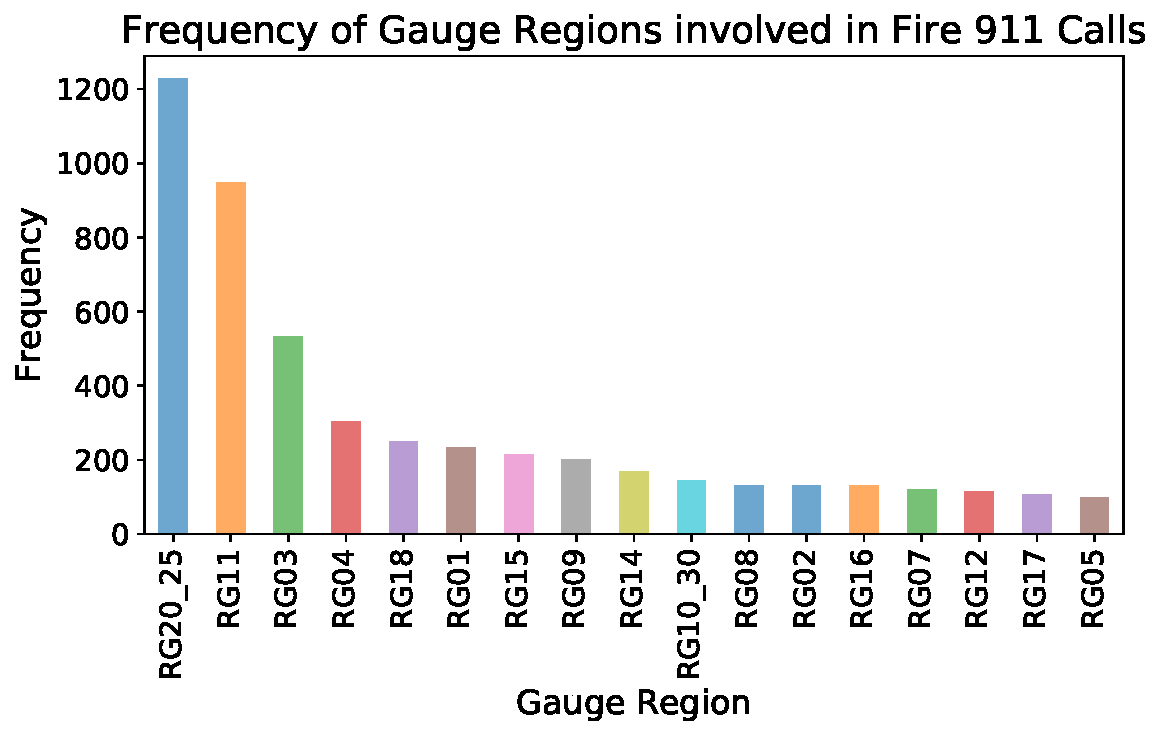
\includegraphics[scale=0.6]{figs/CallsvGauge.pdf}
\caption{Totality of fire 911 calls in each gauge region.}
\label{CallsvGauge}
\end{figure}

As we see, there are some gauge regions that seem to posses an abnormal number of fire 911 calls. In order to be sure that the functions we built to assign the nearest gauge are working, let us make a graphical double check. We can first grab the totality of the original data, plot their frequency using a 2D histogram which follows latitude and longitude as axes. Then we can add the locations of the gauges and directly observe that the anomalies are real. This corresponds to Figure~\ref{2DHist}.

\begin{figure}[ht!]
\centering
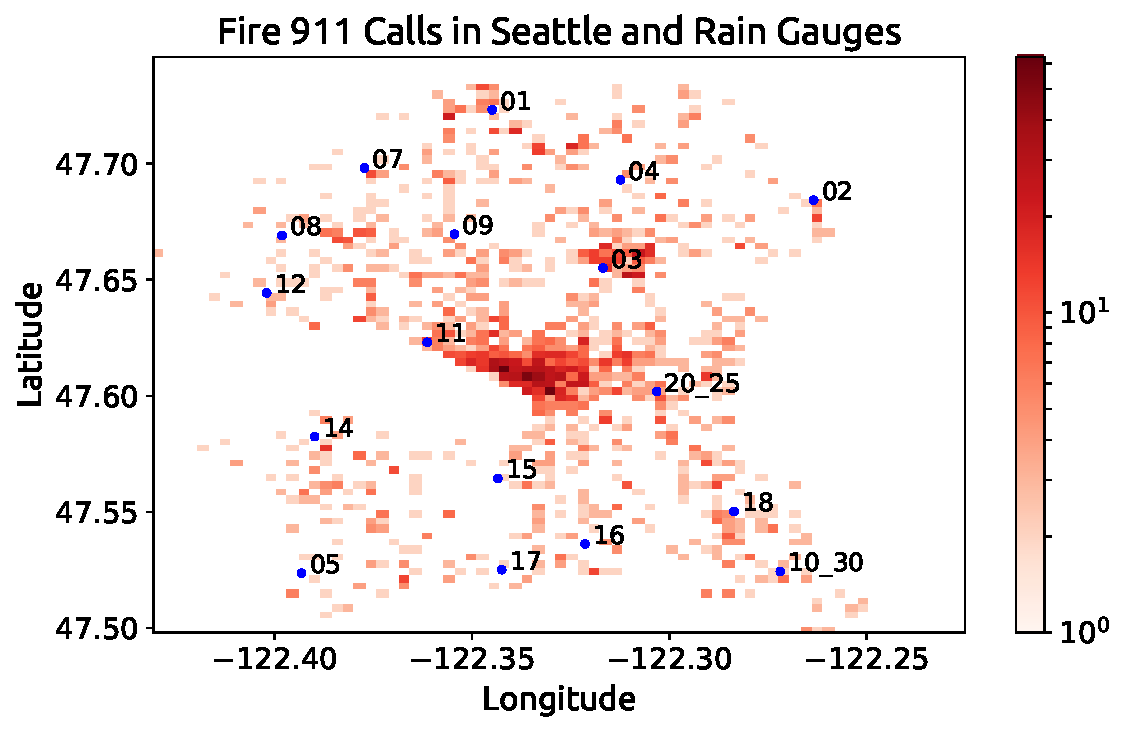
\includegraphics[scale=0.7]{figs/2DHist.pdf}
\caption{Distribution of fire 911 calls in the city of Seattle. In blue we see the locations of the rain gauges of the weather data set.}
\label{2DHist}
\end{figure}

There are indeed accumulations of 911 calls around central Seattle, which explains the excessive counting of calls for specific rain gauges. It is interesting to see how the number of calls is enough to reproduce the coastal line in central Seattle.

Since we are interested in the correlation between calls and rain accumulations, we create a pivot table which aggregates the number of calls for each gauge region and each month. Looking at the set, we find that the months corresponding to 2010-06 and 2011-03 have incomplete data, and therefore we remove them. We can do some basic visualization of this information.

We can directly plot the number of 911 fire calls per gauge region per month, as seen in Figure~\ref{CallsGaugeMonth}. We again find that the gauge regions that we identified previously with abnormal number of calls display this behavior consistently through time.

\begin{figure}[ht!]
\centering
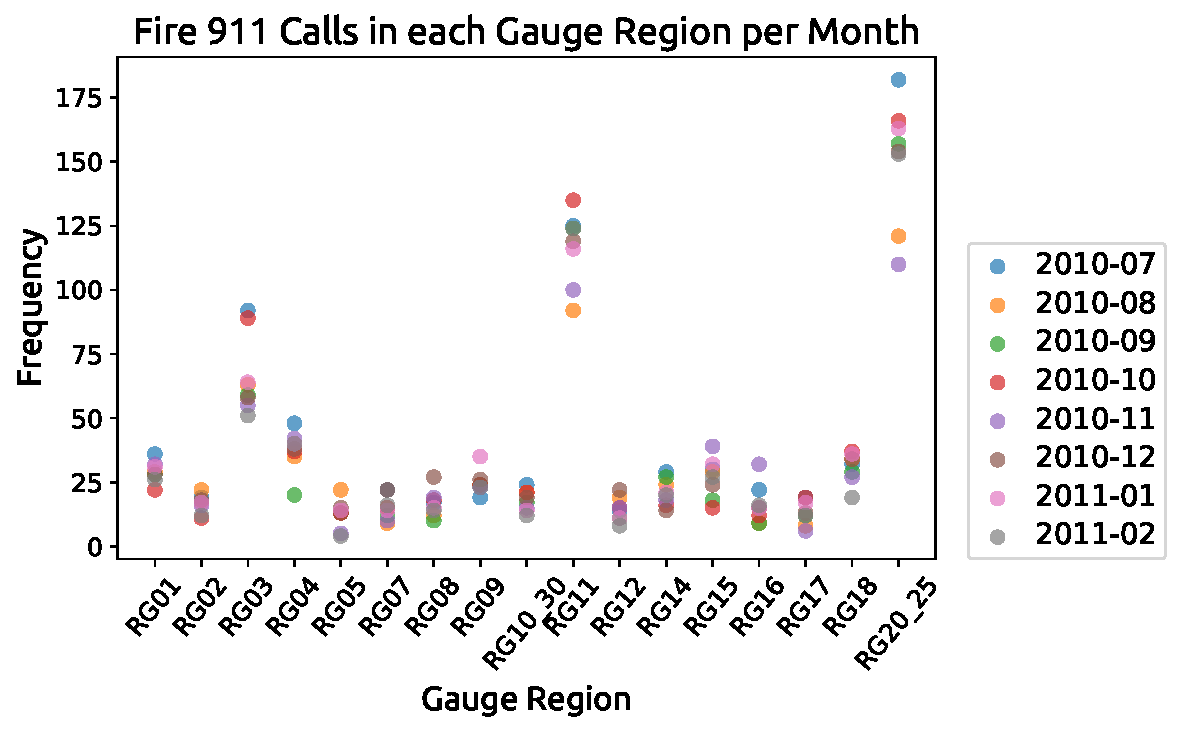
\includegraphics[scale=0.65]{figs/CallsGaugeMonth.pdf}
\caption{Number of fire emergency calls per gauge region, per month. We see again that some sectors present an abnormal number of calls.}
\label{CallsGaugeMonth}
\end{figure}

\subsection{Off days}

With the help of the information in \cite{OfficeHolidays2010,OfficeHolidays2011} on holidays in the state of Washington in 2010 and 2011, we can easily produce a list containing these dates. We store them as \verb|Timestamp| objects that we will be able to relate to the dates in the fire calls data set. We add the weekends to this list in order to complete a list called \verb|off_days|. Saturdays and sundays in a specific year can be produced with \verb|datetime| functions such as \verb|date| and \verb|timedelta|. With these we write a function \verb|all_x_days(x_day,year)|, which provides all the \verb|weekdays = x_day| (e.g. all mondays) in a specific year.

We have in total 231 off days in 2010 and 2011 together, which represents 31.6\% of this period of time. Together with the rain accumulations information, we build a data frame called \verb|df_fire_10_11_off| which contains the data on 911 fire calls together with the rain gauge region and a column that indicates whether the call happened in an off day.

\section{Findings and Analysis}

We explore a couple of potential effects in the manifestation of fire emergencies.

\subsection{Rain and Fire}

Let us consider the possibility of a correlation between rain patterns and number of 911 fire calls. Here we present several pieces of evidence against this hypothesis.

As we found in the EDA process, the gauge regions RG20\_25 and RG05 display the opposite behaviors when it comes to number of fire 911 calls: the former has more than 12 times the number of calls than the latter. If rain was a dominant factor, we would expect a noticeable difference between the rain patterns for these 2 gauges in the dates of relevance. As we see in Figure~\ref{TwoPlots}, this does not seem to be case.

\begin{figure}[ht!]
\centering
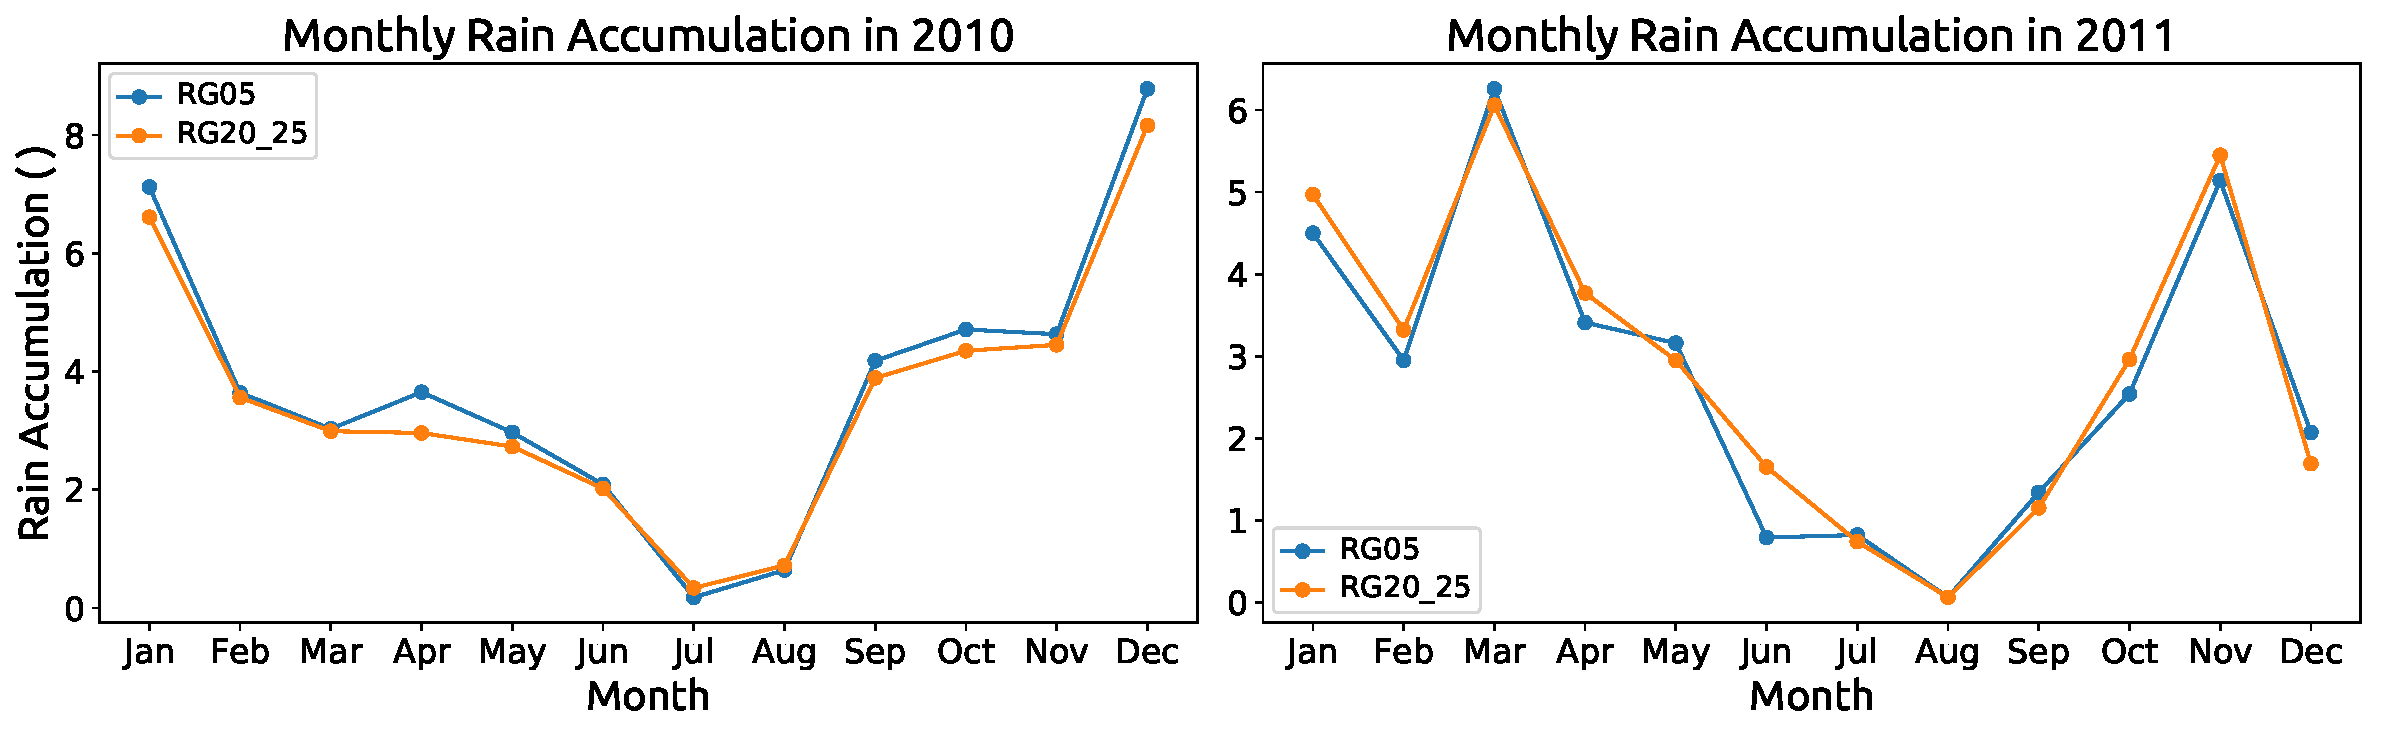
\includegraphics[width=\textwidth]{figs/TwoPlots.pdf}
\caption{Rain accumulations in gauges RG20\_25 and RG05 for the years 2010 (left) and 2011 (right).}
\label{TwoPlots}
\end{figure}

We can certainly find more compelling evidence. We have already organized our data in such a way that we can compare directly number of 911 fire calls and rain accumulation per gauge region per month. We must pair this information which lays in two distinct data frames. Once this is done, we can make a scatter plot of these points, which we see in Figure~\ref{NoCor}.

\begin{figure}[ht!]
\centering
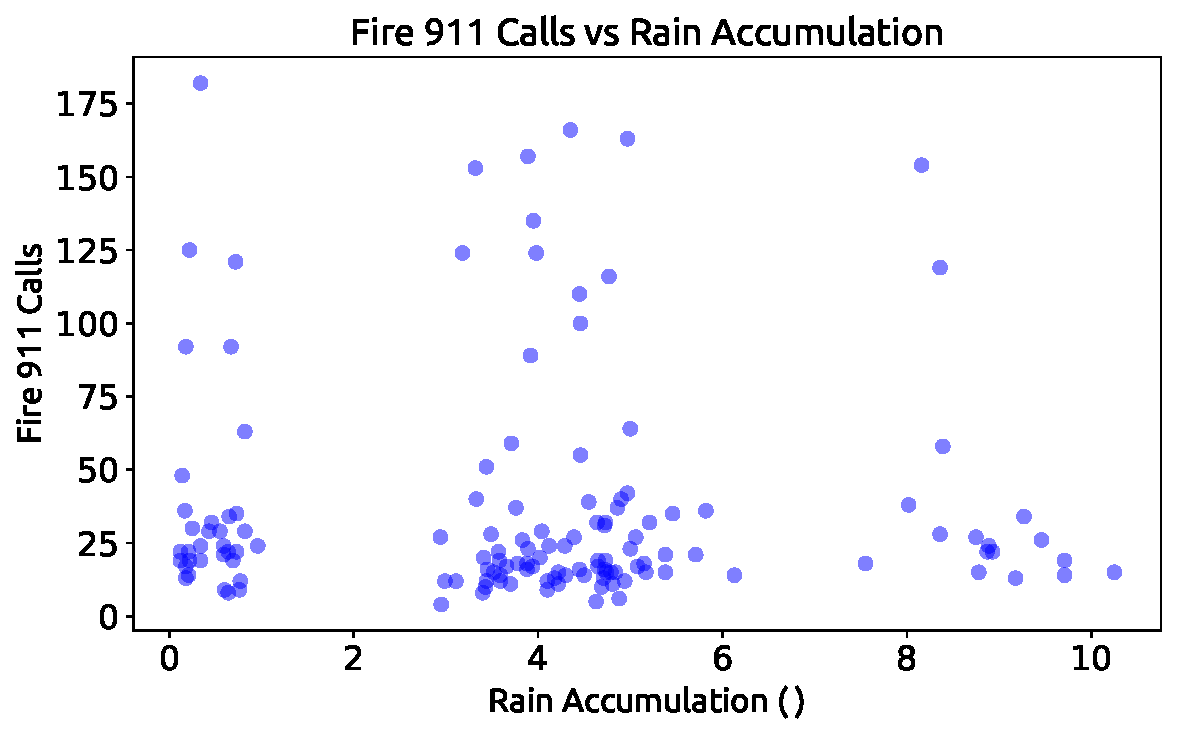
\includegraphics[scale=0.65]{figs/NoCor.pdf}
\caption{Number of fire 911 calls paired with rain accumulations for all the months and rain gauges covered in the data sets.}
\label{NoCor}
\end{figure}

There is little indication of a clear correlation. We also notice that there is a differentiation of rain accumulation in three distinct subgroups. Python corroborates our suspicions,

\begin{verbatim}
stats.linregress(rain_vals, fire_vals)
>> LinregressResult(slope=-0.5492766384107909,
                    intercept=38.98392793888603,
                    rvalue=-0.03588547545789807,
                    pvalue=0.678314825246058,
                    stderr=1.3214179714394578)
\end{verbatim}


The correlation coefficient is -0.036, indicating that there is about 0.1\% of probability of a linear correlation. Even more, the $p$-value indicates that there is a 67.8\% in favor of a null hypothesis for absence of a correlation. This is well beyond any reasonable significance value. There is abundant evidence against the rain patterns being relevant in determining the number of 911 fire calls.

Since we found that the amount of rain accumulation per gauge seems to organize in 3 subgroups, we may be interested in finding the median for the number of 911 calls for each of these 3 subgroups. We may call them points with \emph{reduced}, \emph{medium} and \emph{large} rain accumulations, according to the ranges observed in the $x$ axis of Figure~\ref{NoCor}. The medians are respectively, 24, 19 and 24. Hence, even when slicing the data in these subsets, we can not find a particular behavior that correlates these two variables.

\subsection{Time of the day and Fire}


The previous exploration makes us think that instead of weather conditions, human activity might be the most relevant at exploring 911 fire calls. While we did not found significant difference between month to month data, in these sets we might be able to see whether time of the day plays an important role in the number of 911 calls.

Let us first do a basic counting of \emph{day time} and \emph{night time} calls, by which we will simply mean calls between 6 am and 6 pm for day time and the rest for the night. A first analysis shows a significant abundance of calls in day time relative to the amount of calls in night time. We explore this more clearly by slicing the data hourly.

When we do this, we find an abnormal number of calls in the range between 7 and 8 am. In addition, we found no calls made between 12 pm and 1 am. Due to the difference in orders of magnitude, we do not expect these to be taken as reliable points. For now, we will remove these hours out of our analysis. It is unclear if there is a justification for this odd behavior, which may be due, for instance, to the procedure by which calls are reported or stored at these particular times.

With these corrections taken into account, we find that there are in total 1383 fire emergency calls in day time and 1971 in night time. These numbers show that it is the night time that has more number 911 fire calls after all.

Nevertheless, we should explore the possibility that this is an artifice of the data sample. To study this alternative, we can test this proportion against a null hypothesis of a 50\% amount of night 911 fire calls. To do this we resort to a cumulative binomial distribution and compute the probability of obtaining the observed proportion or higher, assuming the null hypothesis. This $p$-value is of the order of $10^{-24}$, so it is vanishing in practice. This is well below any reasonable level of significance, which suggests we should reject the null hypothesis. This indicates that there are certainly more 911 fire calls in the night. We can see this behavior more clearly in Figure~\ref{TimeOfTheDay}.


\begin{figure}[ht!]
\centering
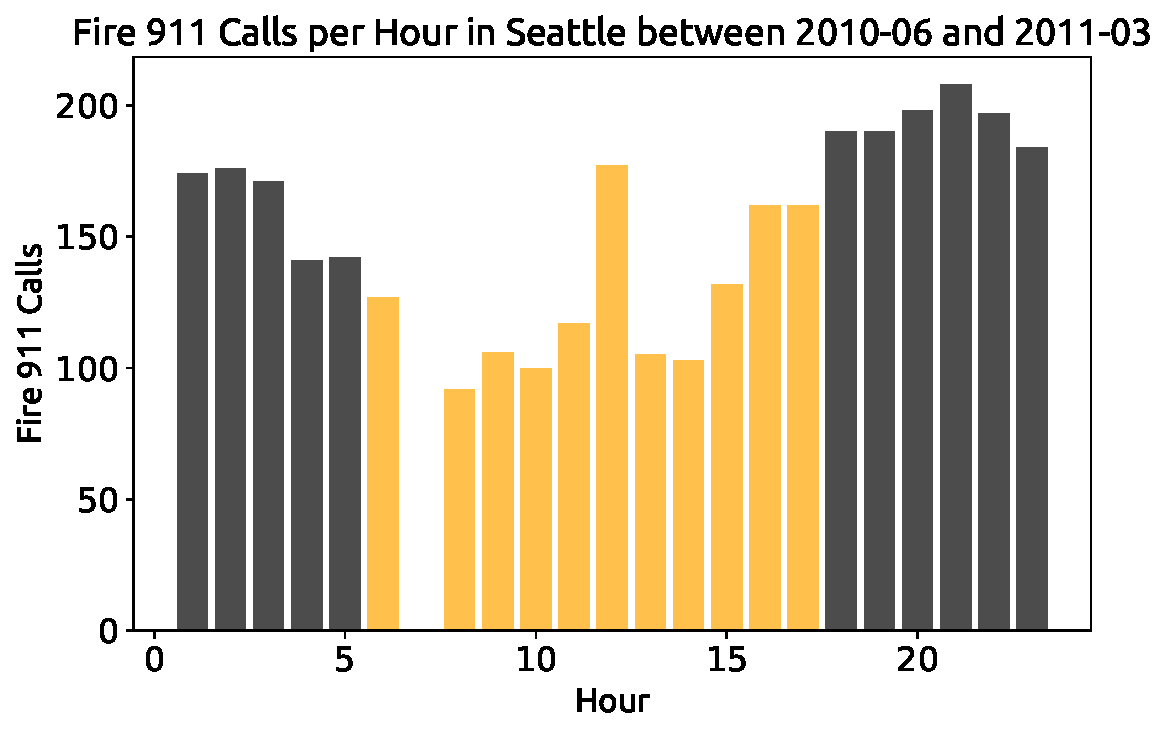
\includegraphics[scale=0.65]{figs/TimeOfTheDay.pdf}
\caption{Number of fire 911 calls grouped by the hour of the call. There is spurious data for the periods between 7 and 8 am and between 12 pm and 1 am, which are hence missing in the plot.}
\label{TimeOfTheDay}
\end{figure}

\subsection{Off days and Fire}

Let us explore the relation between off days and number of emergency calls. We can take a look of the raw number of 911 calls that happened in off days and in regular work days. We find that about 32.1\% of calls happen in off days. This is extremely close to the fraction of off-days to total number of days in 2010 and 2011 that we mentioned before (31.6\%).

It is then reasonable to explore the possibility that the calls in off days simply follow the same proportion that one observes for off days versus the totality of days in 2010 and 2011. We can use this as a null hypothesis for a one-sample proportion test. If the null hypothesis can not be rejected, we would have an indication that whether the days are work days or not does not substantially influence the total number of emergency calls.

By using a cumulative binomial distribution, we find that the probability of the proportion of off day-calls being as extreme or larger than the one we observed under the assumption of the null hypothesis is $p = 0.236$. This is well above any reasonable level of significance, which certainly does not allow us to reject the null hypothesis. This is an indicator that, if the calls are taken as a whole and not split into any categories, there seems to be no influence of the day being a work day or an off day in the number of 911 fire calls.

\section{Machine Learning Analysis}

\cite{Tibshirani}


\section{The Story}

We found no indication that rain accumulations and the number of fire 911 calls are correlated. Fire seems to be more directly related to human activity, as we found that about 53.5\% of the fire emergencies happen in central Seattle. It would be interesting to try to find a correlation of 911 fire calls with population density, if the data were available.

Most of fire emergency calls happen during night time, which seems to reinforce the relevance of human factors over weather. Nevertheless, there is a small peak of activity in the midday, which could match a peak of solar activity. In addition, the proportion of total 911 fire calls is not affected by the day being a work day or not.

Policies for awareness and prevention of fires are a good approach to the reduction of fire related emergencies. These can be focused in fires related to urban activity, specially in highly populated regions of the city, and for events that unfold typically during night time.



%\appendix

%\section{Massive type IIA supergravity} \label{App:MIIA}

\bibliography{references}
%\bibliographystyle{plain}
\bibliographystyle{utphys}


\end{document}